\documentclass[12pt,twoside]{report}
\usepackage{tikz}
\usetikzlibrary{positioning, fit, arrows.meta}
\usepackage{amsmath,amssymb}

%%%%%%%%%%%%%%%%%%%%%%%%%%%%%%%%%%%%%%%%%%%%%%%%%%%%%%%%%%%%%%%%%%%%%%%%%%%%%

% Definitions for the title page
% Edit these to provide the correct information
% e.g. \newcommand{\reportauthor}{Timothy Kimber}

\newcommand{\reporttitle}{Chameleon Text: Exploring ways to increase variety in artificial data}
\newcommand{\reportauthor}{Thien P. Nguyen}
\newcommand{\supervisor}{Lucia Specia}
\newcommand{\degreetype}{Computing (Artificial Intelligence)}

%%%%%%%%%%%%%%%%%%%%%%%%%%%%%%%%%%%%%%%%%%%%%%%%%%%%%%%%%%%%%%%%%%%%%%%%%%%%%

% load some definitions and default packages
%%%%%%%%%%%%%%%%%%%%%%%%%%%%%%%%%%%%%%%%%
% University Assignment Title Page 
% LaTeX Template
% Version 1.0 (27/12/12)
%
% This template has been downloaded from:
% http://www.LaTeXTemplates.com
%
% Original author:
% WikiBooks (http://en.wikibooks.org/wiki/LaTeX/Title_Creation)
%
% License:
% CC BY-NC-SA 3.0 (http://creativecommons.org/licenses/by-nc-sa/3.0/)
% 
%
%%%%%%%%%%%%%%%%%%%%%%%%%%%%%%%%%%%%%%%%%
%----------------------------------------------------------------------------------------
%	PACKAGES AND OTHER DOCUMENT CONFIGURATIONS
%----------------------------------------------------------------------------------------
\usepackage[a4paper,hmargin=2.3cm,vmargin=2.0cm,includeheadfoot]{geometry}
\usepackage{textpos}
\usepackage{natbib} % for bibliography
\usepackage{tabularx,longtable,multirow,subfigure,caption}%hangcaption
\usepackage{fncylab} %formatting of labels
\usepackage{fancyhdr} % page layout
\usepackage{url} % URLs
\usepackage[english]{babel}
\usepackage{amsmath}
\usepackage{graphicx}
\usepackage{dsfont}
\usepackage{epstopdf} % automatically replace .eps with .pdf in graphics
\usepackage{backref} % needed for citations
\usepackage{array}
\usepackage{latexsym}
\usepackage[pdftex,pagebackref,hypertexnames=false,colorlinks]{hyperref} % provide links in pdf

\hypersetup{pdftitle={},
  pdfsubject={}, 
  pdfauthor={},
  pdfkeywords={}, 
  pdfstartview=FitH,
  pdfpagemode={UseOutlines},% None, FullScreen, UseOutlines
  bookmarksnumbered=true, bookmarksopen=true, colorlinks,
    citecolor=black,%
    filecolor=black,%
    linkcolor=black,%
    urlcolor=black}

\usepackage[all]{hypcap}


%\usepackage{color}
%\usepackage[tight,ugly]{units}
%\usepackage{float}
%\usepackage{tcolorbox}
%\usepackage[colorinlistoftodos]{todonotes}
% \usepackage{ntheorem}
% \theoremstyle{break}
% \newtheorem{lemma}{Lemma}
% \newtheorem{theorem}{Theorem}
% \newtheorem{remark}{Remark}
% \newtheorem{definition}{Definition}
% \newtheorem{proof}{Proof}


%%% Default fonts
\renewcommand*{\rmdefault}{bch}
\renewcommand*{\ttdefault}{cmtt}



%%% Default settings (page layout)
\setlength{\parindent}{0em}  % indentation of paragraph

\setlength{\headheight}{14.5pt}
\pagestyle{fancy}
\renewcommand{\chaptermark}[1]{\markboth{\chaptername\ \thechapter.\ #1}{}} 

\fancyfoot[ER,OL]{\sffamily\textbf{\thepage}}%Page no. in the left on odd pages and on right on even pages
\fancyfoot[OC,EC]{\sffamily }
\renewcommand{\headrulewidth}{0.1pt}
\renewcommand{\footrulewidth}{0.1pt}
\captionsetup{margin=10pt,font=small,labelfont=bf}


%--- chapter heading

\def\@makechapterhead#1{%
  \vspace*{10\p@}%
  {\parindent \z@ \raggedright \sffamily
    \interlinepenalty\@M
    \Huge\bfseries \thechapter \space\space #1\par\nobreak
    \vskip 30\p@
  }}

%---chapter heading for \chapter*  
\def\@makeschapterhead#1{%
  \vspace*{10\p@}%
  {\parindent \z@ \raggedright
    \sffamily
    \interlinepenalty\@M
    \Huge \bfseries  #1\par\nobreak
    \vskip 30\p@
  }}

\allowdisplaybreaks

% load some macros
% Here, you can define your own macros. Some examples are given below.

\newcommand{\R}[0]{\mathds{R}} % real numbers
\newcommand{\Z}[0]{\mathds{Z}} % integers
\newcommand{\N}[0]{\mathds{N}} % natural numbers
\newcommand{\C}[0]{\mathds{C}} % complex numbers
\renewcommand{\vec}[1]{{\boldsymbol{{#1}}}} % vector
\newcommand{\mat}[1]{{\boldsymbol{{#1}}}} % matrix


\date{May 2019}

\begin{document}

% load title page
% Last modification: 2015-08-17 (Marc Deisenroth)
\begin{titlepage}

\newcommand{\HRule}{\rule{\linewidth}{0.5mm}} % Defines a new command for the horizontal lines, change thickness here


%----------------------------------------------------------------------------------------
%	LOGO SECTION
%----------------------------------------------------------------------------------------


\includegraphics[width = 4cm]{./figures/imperial}\\[0.5cm] 

\center % Center remainder of the page

%----------------------------------------------------------------------------------------
%	HEADING SECTIONS
%----------------------------------------------------------------------------------------

\textsc{\Large Imperial College London}\\[0.5cm] 
\textsc{\large Department of Computing}\\[0.5cm] 

%----------------------------------------------------------------------------------------
%	TITLE SECTION
%----------------------------------------------------------------------------------------

\HRule \\[0.4cm]
{ \huge \bfseries \reporttitle}\\ % Title of your document
\HRule \\[1.5cm]
 
%----------------------------------------------------------------------------------------
%	AUTHOR SECTION
%----------------------------------------------------------------------------------------

\begin{minipage}{0.4\textwidth}
\begin{flushleft} \large
\emph{Author:}\\
\reportauthor % Your name
\end{flushleft}
\end{minipage}
~
\begin{minipage}{0.4\textwidth}
\begin{flushright} \large
\emph{Supervisor:} \\
\supervisor % Supervisor's Name
\end{flushright}
\end{minipage}\\[4cm]


%----------------------------------------------------------------------------------------
%	FOOTER & DATE SECTION
%----------------------------------------------------------------------------------------
\vfill % Fill the rest of the page with whitespace
Submitted in partial fulfillment of the requirements for the MSc degree in
\degreetype~of Imperial College London\\[0.5cm]

\makeatletter
\@date 
\makeatother


\end{titlepage}



% page numbering etc.
\pagenumbering{roman}
\clearpage{\pagestyle{empty}\cleardoublepage}
\setcounter{page}{1}
\pagestyle{fancy}

%%%%%%%%%%%%%%%%%%%%%%%%%%%%%%%%%%%%
% \begin{abstract}
% Your abstract.
% \end{abstract}

% \cleardoublepage
%%%%%%%%%%%%%%%%%%%%%%%%%%%%%%%%%%%%
% \section*{Acknowledgments}
% Comment this out if not needed.

% \clearpage{\pagestyle{empty}\cleardoublepage}

%%%%%%%%%%%%%%%%%%%%%%%%%%%%%%%%%%%%
%--- table of contents
% \fancyhead[RE,LO]{\sffamily {Table of Contents}}
% \tableofcontents 


% % \clearpage{\pagestyle{empty}\cleardoublepage}
\pagenumbering{arabic}
\setcounter{page}{1}
\fancyhead[LE,RO]{\slshape \rightmark}
\fancyhead[LO,RE]{\slshape \leftmark}

%%%%%%%%%%%%%%%%%%%%%%%%%%%%%%%%%%%%
% \chapter{Introduction}

% \begin{figure}[tb]
% \centering
% 
\includegraphics[width = 0.4\hsize]{./figures/imperial}
% \caption{Imperial College Logo. It's nice blue, and the font is quite stylish. But you can choose a different one if you don't like it.}
% \label{fig:logo}
% \end{figure}

% Figure~\ref{fig:logo} is an example of a figure. 

%%%%%%%%%%%%%%%%%%%%%%%%%%%%%%%%%%%%
\chapter{Literature Survey}

\section{Background}

\subsection{Neural Networks}

Neural Networks are non-linear statistical models that generate complex relationships between input and output vectors. Note that the input and output vectors are of a fixed dimension, which becomes a problem for our task at hand.

\subsection{Backpropagation}

\subsection{Autoencoders}

Autoencoders are a specialised form of MLPs where the model attempts to recreate the inputs on the output. Autoencoders typically have a neural network layer in the model where its dimension is smaller than the input space, therefore representing a dimensionality reduction in the data. Autoencoders are composed of two different principal components, an encoder network $\alpha$ and a decoder network $\beta$, such that $\alpha : X \rightarrow F$ and $\beta : F \rightarrow X$. Measuring the success of the reconstruction is deduced by a reconstruction loss formula. This reconstruction loss comapres the output of the decoder and compares it against the input of the encoder. The two networks are trained together in a manner that allows them to preserve the input as much as possible.

% what is it good for?

Autoencoders are popularised through their use in Machine Translation, Word Embeddings, and document clustering.

% tricks on the autoencoder

denoising autoencoders, where the input is a noisy representation of some input data, and it'll try and remove the noise (by comparing the reconstruction loss against a clean representation of the input).

also shown to have success in reconstructing images via neural inpainting.

\subsection{Recurrent Neural Networks}

Recurrent neural networks (CNNs) are a particular class of neural networks such that the outputs are not necessarily restricted and discrete (as opposed to the MLP). CNNs essentially operate over a sequence of vectors, making them popular in contempoary NLP problems. Given a sequence of inputs $(x_1, ..., x_T)$, a standard RNN computes a sequence of outputs $(y_1, ..., y_T)$ by iterating the following equation:

The semantics, structure and 
It becomes very difficult for RNNs to leverage this; this is described as a long range dependency problem.

\subsubsection{LSTM}

\begin{figure}
	\centering
	\begin{tikzpicture}[
		prod/.style={circle, draw, inner sep=0pt},
		ct/.style={circle, draw, inner sep=5pt, ultra thick, minimum width=10mm},
		ft/.style={circle, draw, minimum width=8mm, inner sep=1pt},
		filter/.style={circle, draw, minimum width=7mm, inner sep=1pt, path picture={\draw[thick, rounded corners] (path picture bounding box.center)--++(65:2mm)--++(0:1mm);
		\draw[thick, rounded corners] (path picture bounding box.center)--++(245:2mm)--++(180:1mm);}},
		mylabel/.style={font=\scriptsize\sffamily},
		>=LaTeX
		]
	
	\node[ct, label={[mylabel]Cell}] (ct) {$c_t$};
	\node[filter, right=of ct] (int1) {};
	\node[prod, right=of int1] (x1) {$\times$}; 
	\node[right=of x1] (ht) {$h_t$};
	\node[prod, left=of ct] (x2) {$\times$}; 
	\node[filter, left=of x2] (int2) {};
	\node[prod, below=5mm of ct] (x3) {$\times$}; 
	\node[ft, below=5mm of x3, label={[mylabel]right:Forget Gate}] (ft) {$f_t$};
	\node[ft, above=of x2, label={[mylabel]left:Input Gate}] (it) {$i_t$};
	\node[ft, above=of x1, label={[mylabel]left:Output Gate}] (ot) {$o_t$};
	
	\foreach \i/\j in {int2/x2, x2/ct, ct/int1, int1/x1,
				x1/ht, it/x2, ct/it, ct/ot, ot/x1, ft/x3}
		\draw[->] (\i)--(\j);
	
	\draw[->] (ct) to[bend right=45] (ft);
	
	\draw[->] (ct) to[bend right=30] (x3);
	\draw[->] (x3) to[bend right=30] (ct);
	
	\node[fit=(int2) (it) (ot) (ft), draw, inner sep=0pt] (fit) {};
	
	\draw[<-] (fit.west|-int2) coordinate (aux)--++(180:7mm) node[left]{$x_t$};
	\draw[<-] ([yshift=1mm]aux)--++(135:7mm);
	\draw[<-] ([yshift=-1mm]aux)--++(-135:7mm);
	
	\draw[<-] (fit.north-|it) coordinate (aux)--++(90:7mm) node[above]{$x_t$};
	\draw[<-] ([xshift=1mm]aux)--++(45:7mm);
	\draw[<-] ([xshift=-1mm]aux)--++(135:7mm);
	
	\draw[<-] (fit.north-|ot) coordinate (aux)--++(90:7mm) node[above]{$x_t$};
	\draw[<-] ([xshift=1mm]aux)--++(45:7mm);
	\draw[<-] ([xshift=-1mm]aux)--++(135:7mm);
	
	\draw[<-] (fit.south-|ft) coordinate (aux)--++(-90:7mm) node[below]{$x_t$};
	\draw[<-] ([xshift=1mm]aux)--++(-45:7mm);
	\draw[<-] ([xshift=-1mm]aux)--++(-135:7mm);
	\end{tikzpicture}
	\caption{A diagram of the LSTM model.}
\end{figure}

LSTM (Long Short Term Memory) is a type of Recurrent Neural Network that attempts to retain information based on the previous inputs through the introduction of gated architectures.

\subsubsection{Gated Recurrent Networks}

GRUs are used to solve the common issue with LSTMs where the training time was relatively slow due to the number of derivatives necessary to compute. Within the GRU architecture, a feature to retain the previous weights remain, but there exists an direct path to the input data from the output, allowing a reduction in training time.

\section{Related Work}

\subsection{Seq2Seq}

Seq2Seq, introduced by \cite{sutskever_sequence_2014} is a modern interpretation of the encoder model, by providing an attention mechanism. The attention mechanism looks at all of the inputs from the hidden states of the encoders so far. 

Traditionally, Seq2seq would be the most common method of tackling this particular problem, but it also presents problems that make it suboptimal. Firstly, it's discrete nature suggests that it is prone to noise in a similar fashion to how linear regression is not necessarily optimal as opposed to 

\subsection{Transformers}

\begin{figure}[!ht]
      
	\centering
	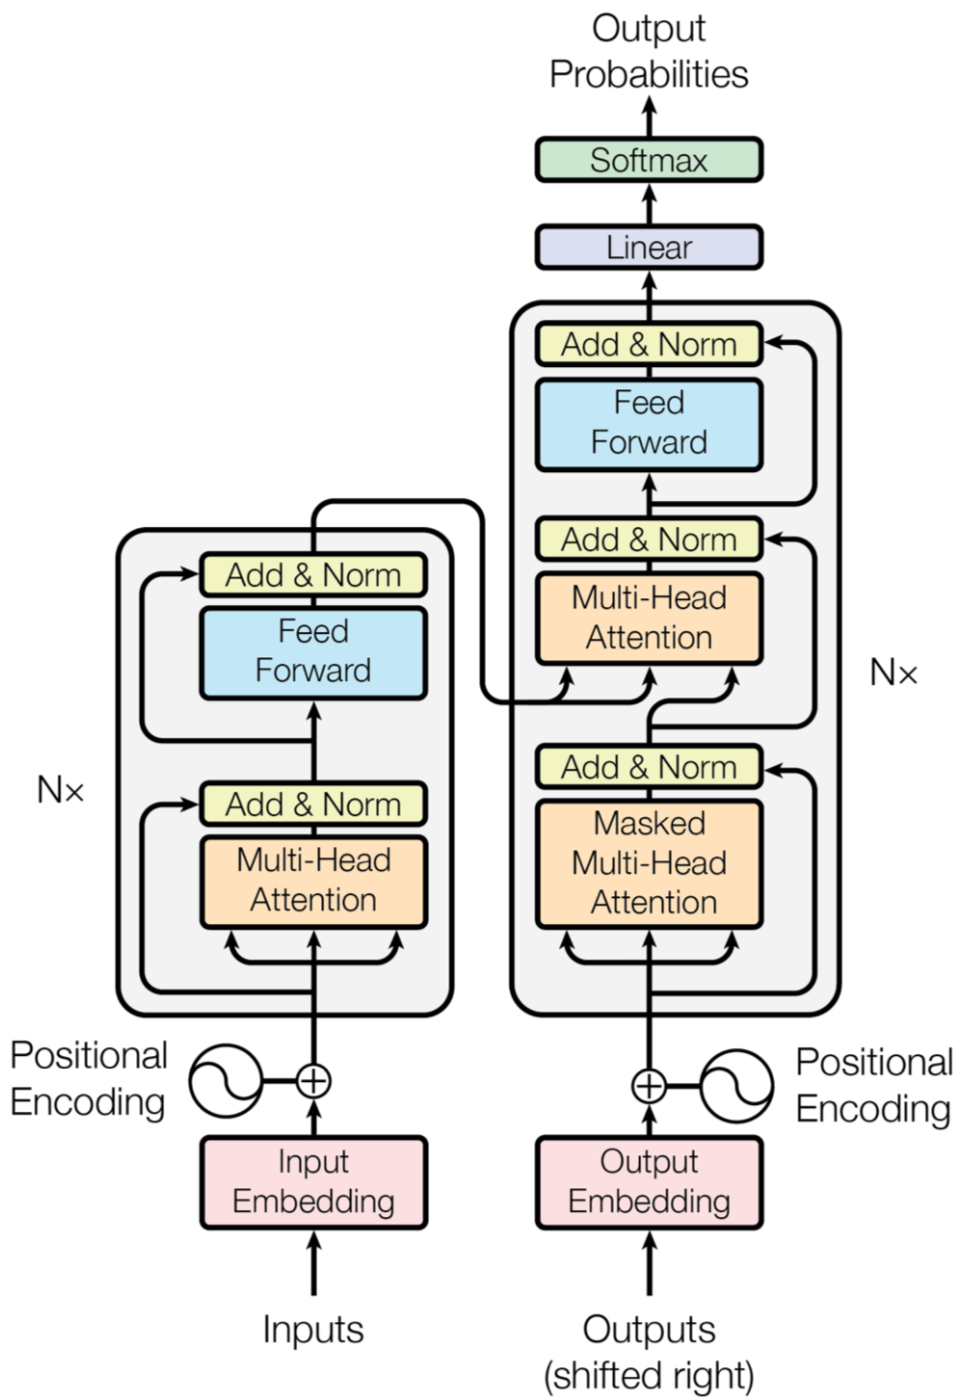
\includegraphics[width=60mm]{diagrams/transformers.png}
	\caption{The transformer model architecture.\cite{vaswani_attention_2017} \label{transformer}}
  \end{figure}

\cite{vaswani_attention_2017} introduced the idea that it is possible to avoid the use of RNNs altogether and focus on leveraging the attention mechanism introduced in seq2seq. The resulting network architecture utilises stacked layers of residual networks 

\subsection{Variational Autoencoders}

Variational Autoencoders (VAEs) introduce a constraint on the encoding network that forces the model to generate latent vectors that roughly follow a gaussian distribution, as opposed to creating a fixed latent vector. Consequently, VAEs introduce two extra vectors, a mean vector and a standard distribution vector, which is fed from the encoder. A sample is taken from the distribution and that is then fed into the decoder.

\begin{figure}[!ht]
      
	\centering
	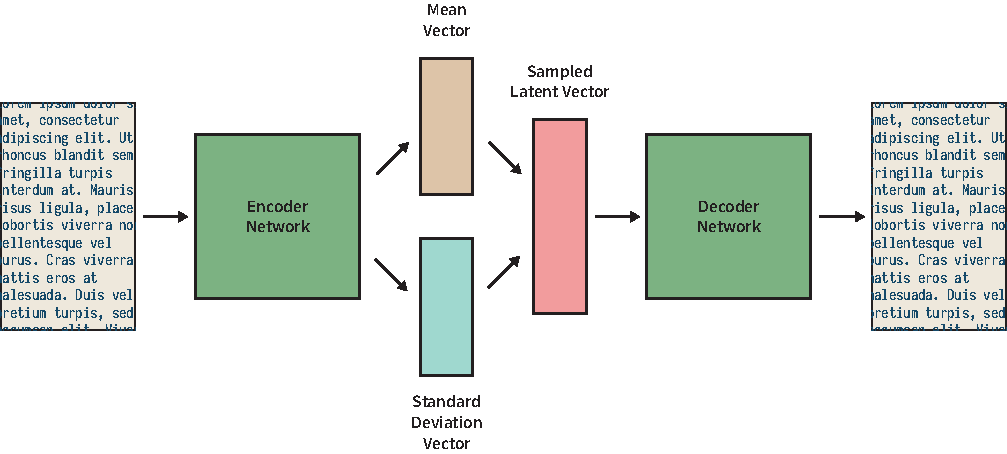
\includegraphics[width=150mm]{diagrams/variational_autoencoders.pdf}
	\caption{A simplified model architecture for a variational autoencoder, which takes as input some text, and it's predicted output being the same text as the input.\label{vae}}
  \end{figure}

  Note that the decoder receives samples from a non-standard normal distribution produced by the encoder. The average of the samples of the different distributions should approximate to a standard normal.
  
  Due to the stochastic nature of the network, we use a reconstruction loss that involves an expection of the output; but we also use the KL divergence, which  measures the relative difference of two probability distributions. In this particular case, we will be comparing the distribution of the decoder outputs against a standard gaussian $ \mathcal{N}(0,1)$).
  
  $$\mathcal{L}(\theta, \phi, x, z) = \mathbb{E}_{q \phi (z|x)}[log \thinspace p_{\theta}(x|z)] - D_{KL}(q_{\phi}(z|x)\thinspace||\thinspace p(z)) $$

$$
D_{KL}(P ||Q) = \sum_{x \subset X} P(x) \cdot log (\frac{P(x)}{Q(x)})
$$

In other words, it is the expectation of the logarithmic difference between the probabilities $P$ and $Q$, where the expectation of $P$ is understood.


- You'll need to perform a reparameterisation trick (since you can't calculate derivatives of samples.) in order to perform backpropagation. (you can't push gradients through a sampling node.)
  
$$z = \mu + \sigma \cdot \epsilon $$ where $\epsilon \sim \mathcal{N}(0,1)$. You want to learn $\mu, \sigma$.



\subsection{Conditional Variational Autoencoders}

Although VAEs are more robust when compared to their original autoencoder counterparts, the decoder class cannot produce outputs of a particular class on demand. CVAEs are an improved model of the original VAE architecture by conditioning on another description of the data, a class descriptor $y$. 

\begin{figure}[!ht]
      
	\centering
	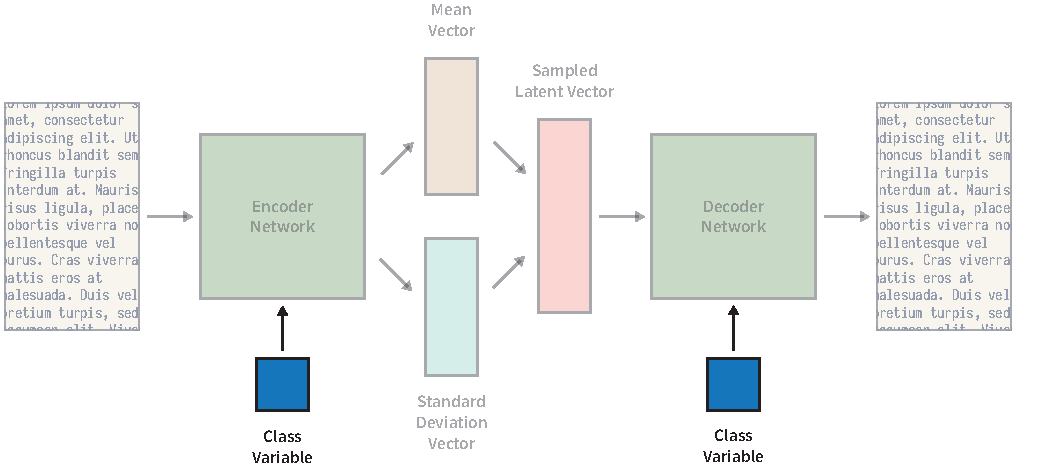
\includegraphics[width=150mm]{diagrams/conditional_variational_autoencoders.pdf}
	\caption{A model architecture for a CVAE, which includes the label being fed into the encoder and decoder networks. \label{cvae_diagram}}
  \end{figure}

During training time, a class (represented by some arbitary vector) is fed at the same time to the encoder and decoder. To generate an output that depends on $y$ we feed that number to the decoder along with a random point in the latent space sampled from a standard normal distribution.

Samples can be generated from the conditional distribution $p(x|y)$. By changing the value of $y$, we can get corresponding samples $x \sim p(x|y)$. The system no longer relies on the latent space to encode what output is necessary; instead the latent space encodes other information that can distinguish itself based on the differing $y$ values.

However, it was found by \cite{du_variational_2018} that since the responses were generated from the same latent variable (induced by the class), it was not necessarily sufficent to model high-variability in responses.

\subsection{Variational Autoregressive Decoders}

Introduced by \cite{du_variational_2018}, Variational Autoregressive Decoders (VADs) attempt to circumvent the sampling problem introduced from CVAEs by introducing latent variables in a autoregressive Decoder. At different time-steps, this allows the decoder to produce a multimodal distribution of text sequences, allowing a variety of responses to be produced. It applies bayesian statistics to 

% %%%%%%%%%%%%%%%%%%%%%%%%%%%%%%%%%%%%
% \chapter{Contribution}


% %%%%%%%%%%%%%%%%%%%%%%%%%%%%%%%%%%%%
% \chapter{Experimental Results}


% %%%%%%%%%%%%%%%%%%%%%%%%%%%%%%%%%%%%
% \chapter{Conclusion}


%% bibliography
\bibliographystyle{apa}
\bibliography{ref} 

\end{document}
